\section{Results}

\subsection{System Dynamics SIR Simulation}
TODO: SIR dynamics using SD with FrABS, using 1.0, 0.5, 0.1 and 0.01 sampling 

\begin{figure}
	\centering
	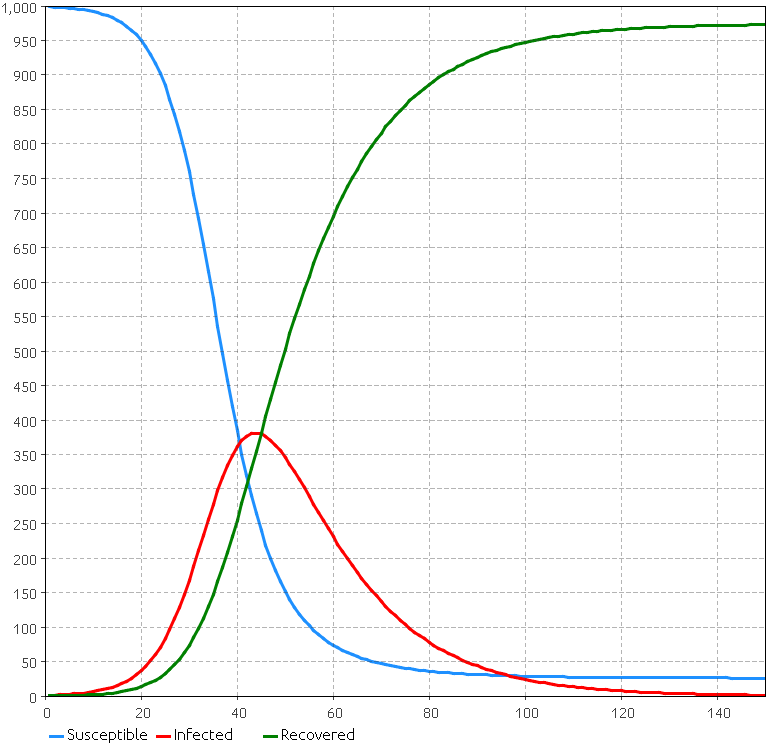
\includegraphics[width=.4\textwidth, angle=0]{./../shared/fig/SIR_SD_DYNAMICS_ANYLOGIC.png}
	\caption{Dynamics of the SIR compartment model using the System Dynamics approach generated with generated with AnyLogic Personal Learning Edition 8.1.0. Population Size $N$ = 1000, contact rate $\beta = 1/5$, infectivity $\gamma = 0.05$, illness duration $\delta = 15$ with initially 1 infected agent, run for 150 time-units.}
	\label{fig:sir_sd_dynamics_anylogic}
\end{figure}

\begin{figure*}
\begin{center}
	\begin{tabular}{c c}
		\begin{subfigure}[b]{0.5\textwidth}
			\centering
			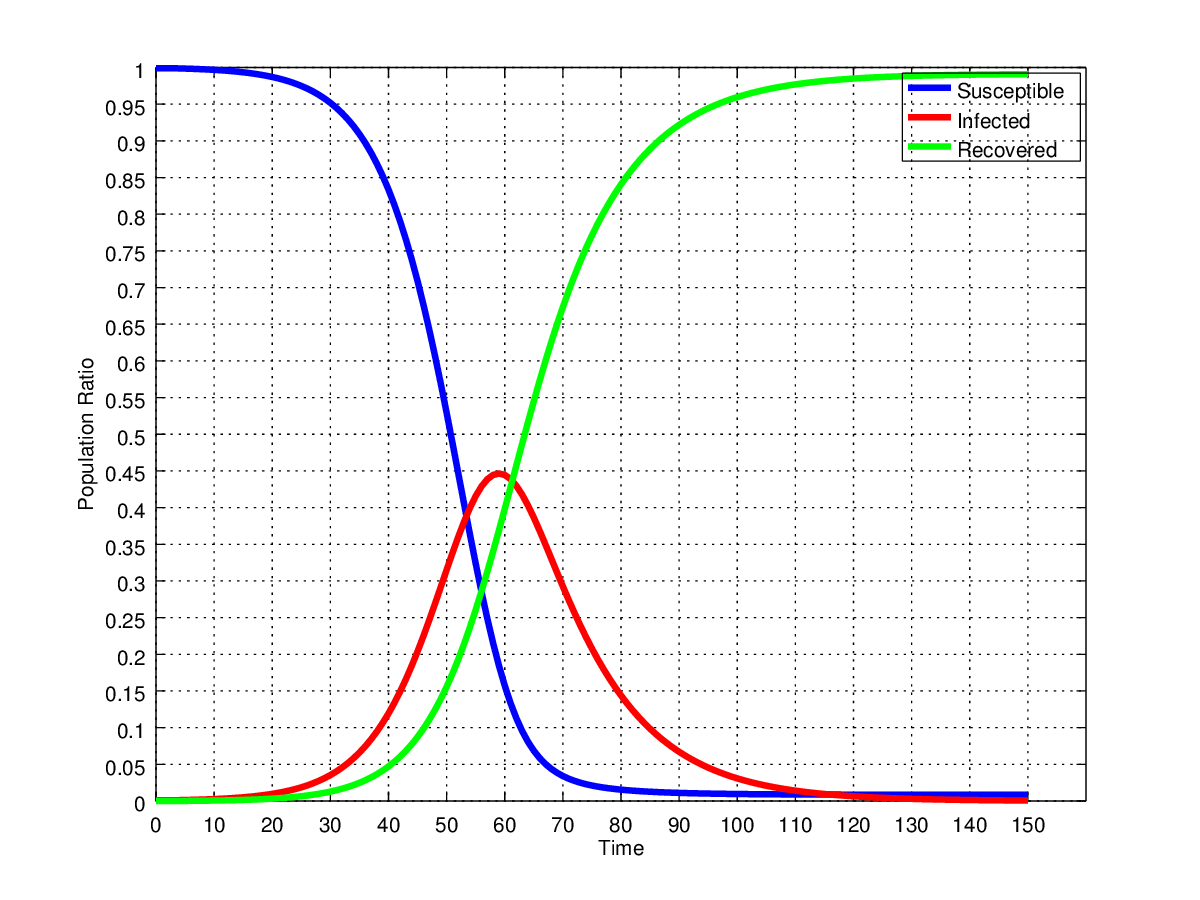
\includegraphics[width=.7\textwidth, angle=0]{./../shared/fig/SIR_SD_DYNAMICS_1000Agents_10dt.png}
			\caption{$\Delta$ 1.0}
			\label{fig:pd_seq}
		\end{subfigure}
    	&
		\begin{subfigure}[b]{0.5\textwidth}
			\centering
			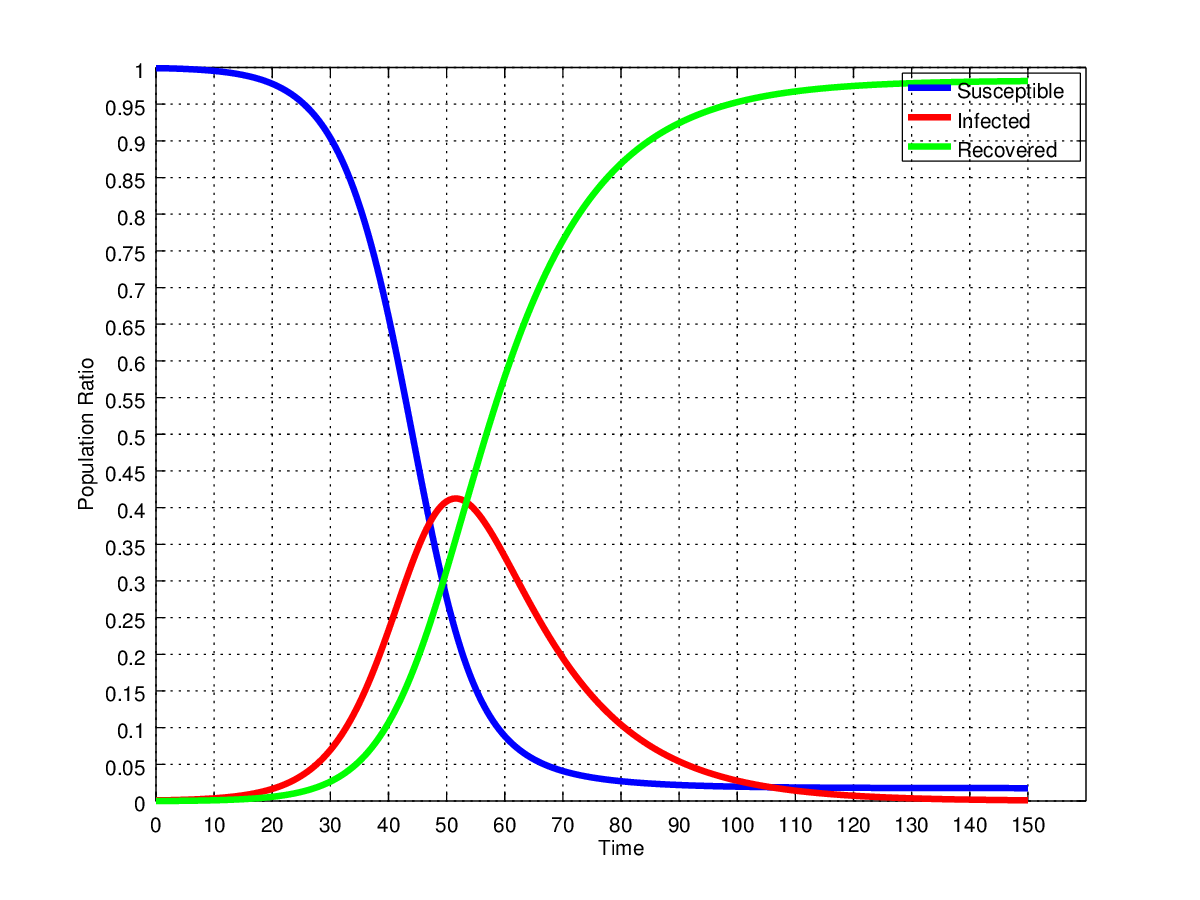
\includegraphics[width=.7\textwidth, angle=0]{./../shared/fig/SIR_SD_DYNAMICS_1000Agents_05dt.png}
			\caption{$\Delta$ 0.5}
			\label{fig:pd_seq}
		\end{subfigure}
    	
    	\\
    	
		\begin{subfigure}[b]{0.5\textwidth}
			\centering
			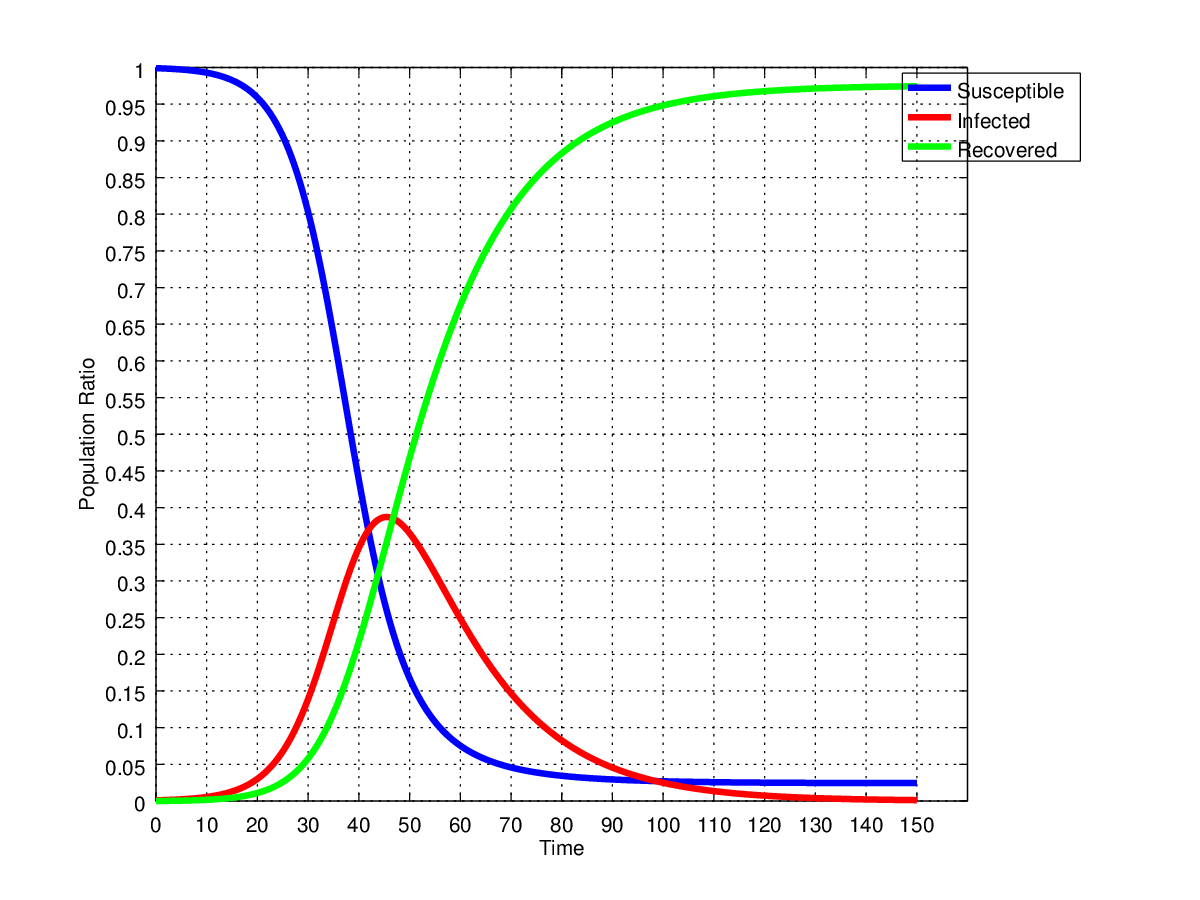
\includegraphics[width=.7\textwidth, angle=0]{./../shared/fig/SIR_SD_DYNAMICS_1000Agents_01dt.png}
			\caption{$\Delta$ 0.1}
			\label{fig:hac_seq}
		\end{subfigure}
		&
		\begin{subfigure}[b]{0.5\textwidth}
			\centering
			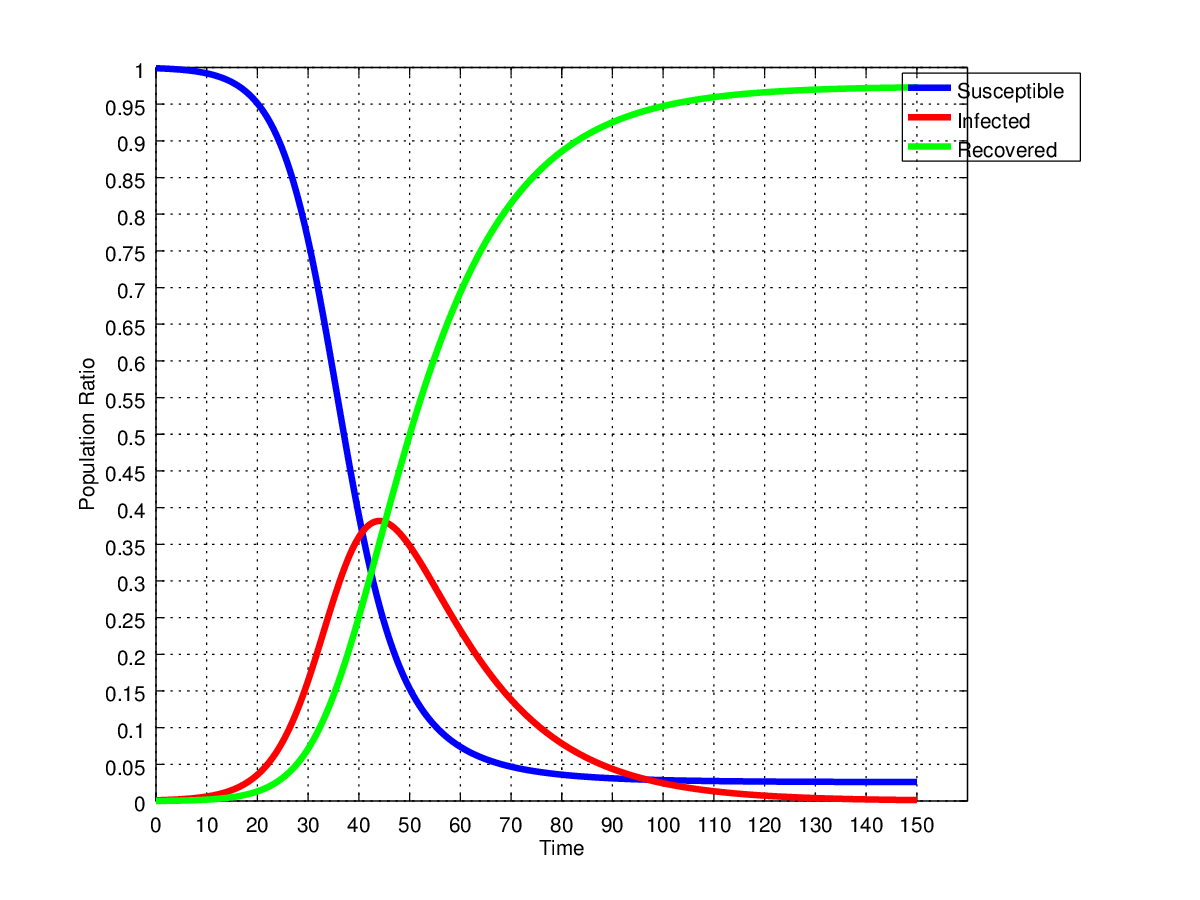
\includegraphics[width=.7\textwidth, angle=0]{./../shared/fig/SIR_SD_DYNAMICS_1000Agents_001dt.png}
			\caption{$\Delta$ 0.01}
			\label{fig:hac_seq}
		\end{subfigure}
	\end{tabular}
	
	\caption{Dynamics of the SIR compartment model using the System Dynamics approach generated with generated with FrABS with the same model parameters as in Figure \ref{fig:sir_sd_dynamics_anylogic} (population Size $N$ = 1000, contact rate $\beta = 1/5$, infectivity $\gamma = 0.05$, illness duration $\delta = 15$ with initially 1 infected agent, run for 150 time-units.).} 
	\label{fig:sir_sd_dynamics_frabs}
\end{center}
\end{figure*}

\subsection{Agent-based SIR Simulation}
TODO: SIR dynamics using ABS with FrABS, using 1.0, 0.5, 0.1 and 0.05 sampling with 1000 agents

TODO: need to do the same thing as AnyLogic. maybe the problem is sampling as well as replications as number of agents, which leaves us in a pretty bad shape performance wise.
	-> how many agents? are 1000 enough?
	-> how many replications? are 32 enough?
	-> what is the sampling interval? 0.1 enough or do we have to go below?
	1000 agents with 16 replications and 0.05 dt seems to deliver pretty good results
	need enough initially infected agents, otherwise wouldn't work

